\chapter{الاعداد المرڪبة}

\section{الجمع والضرب} 
\textbf{\textit{الاعداد المرڪبة}} تعرف بأنها الازواج المرتبة $(x, y)$ من الاعداد الحقيقية والتي نتعامل معها ڪنقاط في المستوي.
{
		\begin{tikzpicture}
	\draw[thick, -latex] (0, -0.5) -- (0,4) node[left] {$y$};
	\draw[thick, -latex] (-0.5, 0) -- (6, 0) node[below] {$x$};
	\node[below left] (0, 0) {$O$};
		
		% تعريف الإحداثيات
		\coordinate (Z) at (4,2);
		\coordinate (I) at (0,1);
		\coordinate (X) at (4,0);
		
		% رسم النقاط
		\filldraw[thick, black] (Z) circle (2pt);
		\filldraw[thick, black] (I) circle (2pt);
		\filldraw[thick, black] (X) circle (2pt);
		
		% رسم التسميات بعيداً عن النقاط
		\node[right] at (Z) {$z=(x,y)$};
		\node[left]  at (I) {$i=(0,1)$};
		\node[below] at (X) {$x=(x,0)$};
		
\end{tikzpicture}
\FIGURE{}}


\section*{تمارين}
\begin{enumerate}
	\item تحقق من\\
	\begin{tasks*}
		\item $(1+i)(1-i) = 2$
		\item $(2+i)(2-i) = 5$
		\item $(3+2i)(1-2i) = 7-4i$
	\end{tasks*}
	
	\item اثبت ان\\
	\begin{tasks*}
		\item $\re(i z) = - \im z$
		\item $\im(i z) = \re z$
		\item $\re(z^2) = x^2 - y^2$ من اجل $z = x+iy$
		\item $\im(z^2) = 2xy$ من اجل $z = x+iy$
	\end{tasks*}
	
	\item برهن ان 
	\[
	(1 + z)^3 = 1 + 3z + 3z^2 + z^3
	\]
	
	\item اثبت ان كلا العددين 
	\[
	z = i, \quad z = -i
	\] 
	يحققان المعادلة $z^2 + 1 = 0$.
	
	\item حل المعادلة 
	\[
	z^2 - 2z + 5 = 0
	\] 
	من اجل $z = (x, y)$ من خلال كتابة
	\[
	(x, y)(x, y) - 2(x, y) + (5, 0) = (0, 0)
	\]
	ومن ثم حل نظام من المعادلات في $x$ و $y$.
	
	\SUG{استخدم التمثيل البياني للعدد المركب أو حل المعادلة كنظام: $x^2 - y^2 - 2x + 5 = 0$, $2xy - 2y = 0$}
	
	\ANS{$z = (1, \pm 2)$}
	
	\item حل المعادلة 
	\[
	z^3 = 1
	\] 
	واحصل على جميع الجذور من الشكل $z = (x, y)$.
	
	\ANS{
		\[
		z_1 = (1,0), \quad z_2 = \left(-\dfrac{1}{2}, \dfrac{\sqrt{3}}{2}\right), \quad z_3 = \left(-\dfrac{1}{2}, -\dfrac{\sqrt{3}}{2}\right)
		\]
	}
	
	\item \begin{tasks*}
		\item اوجد الناتج: $(2+3i) + (1-4i)$
		\ANS{$3 - i$}
		
		\item اوجد الناتج: $(1+i)(1-i)$
		\ANS{$2$}
		
		\item اوجد الناتج: $(3+i)^2$
		\ANS{$8 + 6i$}
		
		\item اوجد الناتج: $\dfrac{2+3i}{1-i}$
		\ANS{$\dfrac{-1+5i}{2}$}
	\end{tasks*}
\end{enumerate}

\section{بعض الخواص الجبرية}

\section*{تــماريــن}
\begin{enumerate}
	\item بسط المقادير التالية الى ابسط صورة\\
	\begin{tasks}
		\item $\dfrac{1+2i}{3-4i} + \dfrac{2-i}{5i}$ ؛ 
		\item $\dfrac{5i}{(1-i)(2-i)(3-i)}$ ؛ 
		\item $(1-i)^4$
	\end{tasks}\\[10pt]
	\ANS{
	\begin{tasks}
		\item $-2/5$ ؛
		\item $-1/2$ ؛ 
		\item $-4$
	\end{tasks}
	}
	\item اثبت أن
	\[
	\frac{1}{1/z} = z \qquad (z\neq 0)
	\]
	
	\item استعمل قواعد التجميع والتوزيع لعملية الضرب لتبرهن أن
	\[
	(z_1 z_2)(z_3 z_4) = (z_1 z_3)(z_2 z_4)
	\]
\end{enumerate}

\section{المزيد من الخواص الجبرية}

\section{المتجهات والمعيار}



{\noindent
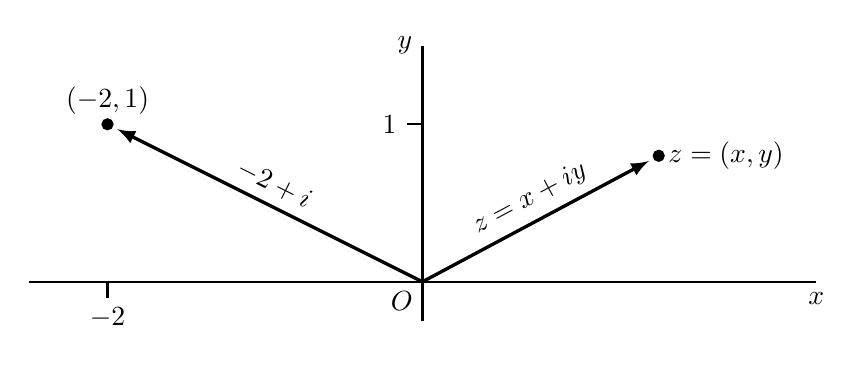
\begin{tikzpicture}[scale=2]
		\draw[thick] (-2.5, 0) -- (2.5, 0) node[below] {$x$};
		\draw[thick] (0, -0.25) -- (0, 1.5) node[left] {$y$};

		\node[below left] at (0, 0) {$O$};
		
		\draw[thick] (0, 1) -- (-0.1, 1) node[left] {$1$};
		\draw[thick] (-2, 0) -- (-2, -0.1) node[below] {$-2$};
		
		\draw[very thick, -latex, shorten >=4pt] (0, 0) -- node[sloped, above] {$z=x+iy$} (1.5, 0.8);
		
		\draw[fill=black] (1.5, 0.8) circle (1pt) node[right] {$z=(x, y)$};
		
		\draw[very thick, -latex, shorten >=4pt] (0, 0) -- node[sloped, above] {$-2+i$} (-2, 1);
		
		\draw[fill=black] (-2, 1) circle (1pt) node[above] {$(-2,1)$};
\end{tikzpicture}
\FIGURE{}}

{\noindent
\begin{tikzpicture}[scale=2.5]
		\draw[thick] (-0.25, 0) -- (2.6, 0) node[below] {$x$};
		\draw[thick] (0, -0.25) -- (0, 1.8) node[left] {$y$};
		
		\node[below left] at (0, 0) {$O$};
		
		\draw[very thick, -latex, shorten >= 4pt] (0, 0) -- node[left, pos=0.65] {$z_2$} (0.5, 1);
		\draw[very thick, -latex, shorten >= 4pt] (0, 0) -- node[below, pos=0.65]{$z_1$} (1.5, 0.5);
		\draw[very thick, -latex, shorten >= 4pt] (0, 0) --node[sloped, above]{$z_1+z_2$} (2, 1.5);
		
		\draw[fill=black] (0.5, 1) circle (1pt);
		\draw[fill=black] (1.5, 0.5) circle (1pt);
		\draw[fill=black] (2, 1.5) circle (1pt);
		
		\draw[mydash, thick, shorten >=14pt] (0.5, 1) -- (2, 1.5);
		\draw[very thick, mydash, -latex, shorten >=6pt] (1.5, 0.5) -- (2, 1.5);
\end{tikzpicture}
\FIGURE{}}


{\noindent
\begin{tikzpicture}[scale=2.5]
		\draw[thick] (-0.25, 0) -- (2.6, 0) node[below] {$x$};
		\draw[thick] (0, -0.25) -- (0, 1.8) node[left] {$y$};
		
		\node[below left] at (0, 0) {$O$};
		
		\coordinate (O) at (0, 0);
		\coordinate (z1) at (2, 0.5);
		\coordinate (z2) at (0.5, 1);
		\coordinate (z3) at (1.5, -0.5);
		\draw[very thick, -latex, shorten >= 4pt] (O) -- node[left, pos=0.65] {$z_2$} (z2);
		\draw[very thick, -latex, shorten >= 4pt] (O) -- node[below, pos=0.65]{$z_1$} (z1);
		
		
		\draw[fill=black] (z2) circle (1pt) node[above]{$(x_2, y_2)$};
		\draw[fill=black] (z1) circle (1pt) node[right]{$(x_1, y_1)$};
		\draw[fill=black] (z3) circle (1pt);
		
		\draw[mydash, very thick, -latex, shorten >=4pt] (z1) --node[right, pos=0.65]{$-z_2$} (z3);
		\draw[mydash, thick] (z2) --node[sloped, above]{$|z_1-z_2|$} (z1);
		
		\draw[very thick, -latex, shorten >=4pt] (O) --node[sloped, below]{$z_1-z_2$} (z3);
		
\end{tikzpicture}
\FIGURE{}}

\section{المتراجحة المثلثية}

\section{المــُرافق العقدي}

{\noindent
\begin{tikzpicture}[scale=2]
		\draw[thick] (-0.5, 0) -- (2.6, 0) node[below] {$x$};
		\draw[thick] (0, -0.5) -- (0, 1.8) node[left] {$y$};
		\node[below left] at (0, 0) {$O$};
		
		\draw[very thick, -latex, shorten >=4pt] (0, 0) --node[above]{$z$} (1.5, 0.5);
		\draw[very thick, -latex, shorten >=4pt] (0, 0) --node[below]{$\conj{z}$} (1.5, -0.5);
		\draw[thick, mydash] (1.5, 0.5) -- (1.5, -0.5);
		
		\draw[fill=black] (1.5, 0.5) circle (1pt) node[right]{$(x, y)$};
		\draw[fill=black] (1.5, -0.5) circle (1pt) node[right]{$(x, -y)$};
\end{tikzpicture}
\FIGURE{}}

\section{الصيغة الأُسية}

{\noindent
\begin{tikzpicture}[scale=1, thick]
	\draw (-pi+1, 0) -- (pi+1, 0) node[above, pos=0.99]{$x$};
	\draw (0, -2) -- (0, 3) node[left, pos=0.96]{$y$};
	\coordinate (A) at (70:2);
	\draw[fill=black] (A) circle (2pt) node[right]{$z = x+iy$};
	\draw[-latex, 
	shorten >=3pt, very thick
	] (0:0) -- (A);
	\draw (0:.3) arc(0:90:.3 and .4);
	\draw (90:.4) arc(90:180:.5 and .4);
	\draw (180:.5) arc(180:270:.5 and .6);
	\draw (270:.6) arc(270:360:.7 and .6);
	\draw[-latex] (0:.7) arc(0:69:.7) node[right, pos=0.55]{$\theta$};
\end{tikzpicture}
\FIGURE{}}

{\noindent
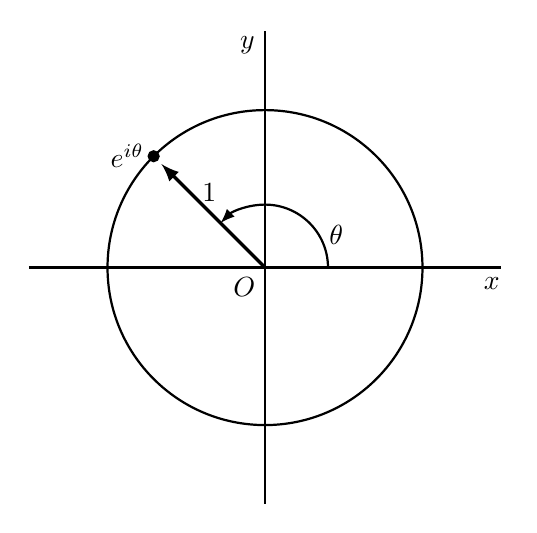
\begin{tikzpicture}[scale=2]
	\draw[thick] (-1.5, 0) -- (1.5, 0) node[below, pos=0.98]{$x$};
	\draw[thick] (0, -1.5) -- (0, 1.5) node[left, pos=0.97]{$y$};
	\node[below left] at (0, 0) {$O$};
	
	\coordinate (A) at (135:1);
	
	\draw[thick] (0:0) circle (1);
	
	\draw[fill=black] (A) circle (1pt) node[left]{$e^{i\theta}$};
	
	\draw[very thick, -latex, shorten >=4pt] (0:0) --node[above]{$1$} (A);
	
	\draw[-latex, thick] (0:0.4) arc(0:135:0.4) node[pos=0.23, right]{$\theta$};
\end{tikzpicture}
\FIGURE{}}

\section{الضرب والقوى في الصيغة الأسية}

\section{السعة للضرب والقسمة}

{\noindent
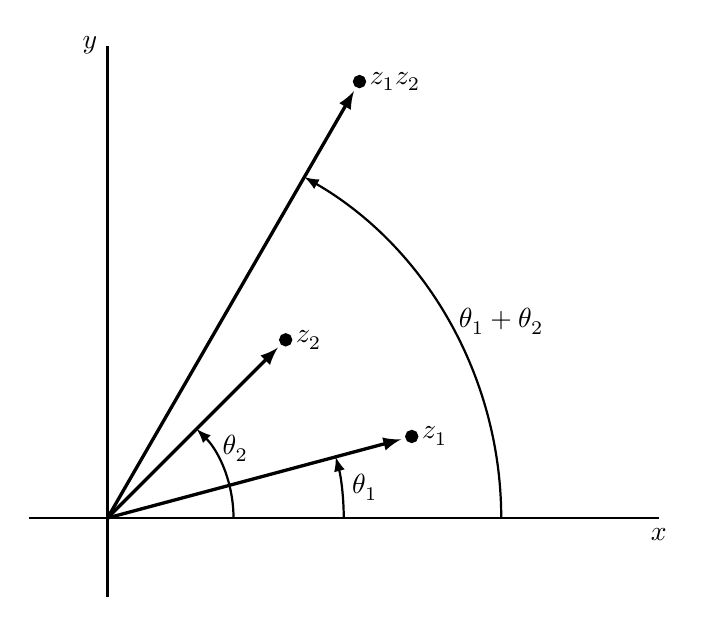
\begin{tikzpicture}[scale=2,thick]
	\draw[thick] (-.5,0)--(3.5,0) node[below]{$x$};
	\draw[thick] (0,-.5)--(0,3) node[left]{$y$};
	\def\aone{15} \def\atwo{45}
	\def\rone{2}  \def\rtwo{1.6}
	\draw[fill=black] (\aone:\rone) circle (1pt) node[right] {$z_1^{}$};
	\draw[fill=black] (\atwo:\rtwo) circle (1pt) node[right] {$z_2^{}$};
	\draw[fill=black] (\aone+\atwo:\rone*\rtwo) circle (1pt) node[right] {$z_1^{}z_2^{}$};
	\draw[very thick, -latex, shorten >=4pt]
	(0,0)--(\aone:\rone);
	\draw[very thick, -latex, shorten >=4pt] (0,0)--(\atwo:\rtwo);
	\draw[very thick, -latex, shorten >=4pt] (0,0)--(\aone+\atwo:\rone*\rtwo);
	\draw[-latex] (0:1.5) arc(0:\aone:1.5) 
	node[pos=.5,right]{$\theta_1^{}$};
	\draw[-latex] (0:.8) arc(0:\atwo:.8) 
	node[pos=.75,right]{$\theta_2^{}$};
	\draw[-latex] (0:2.5) arc(0:\aone+\atwo:2.5)
	node[pos=.5,right]{$\theta_1^{}+\theta_2^{}$};
\end{tikzpicture}
\FIGURE{}}

\section{جذور الاعداد العقدية}

{\noindent
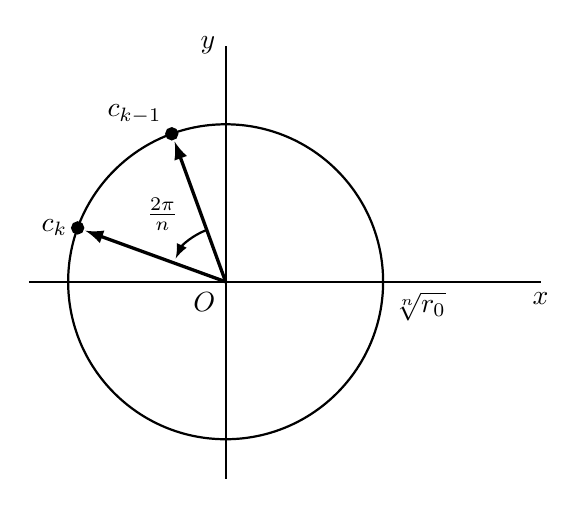
\begin{tikzpicture}[thick]
	\draw[] (-2.5, 0) -- (4, 0) node[below]{$x$};
	\draw[] (0, -2.5) -- (0, 3) node[left]{$y$};
	\draw[] (0, 0) circle (2);
	\node[below left] at (0, 0) {$O$};
	\node[below right] at (0:2) {$\sqrt[n]{r_0}$};
	\coordinate (A) at (110:2);
	\coordinate (B) at (160:2);
	\draw[fill=black] (A) circle (2pt) node[above left]{$c_{k-1}$};
	\draw[fill=black] (B) circle (2pt) node[left]{$c_k$};
	\draw[very thick, -latex, shorten >=3pt] (0, 0) -- (A);
	\draw[very thick, -latex, shorten >=3pt] (0, 0) -- (B);
	\draw[-latex] (110:0.7) arc(110:155:0.7) node[pos=0.5, above left]{$\frac{2\pi}{n}$};
\end{tikzpicture}
\FIGURE{}}

{\noindent
\begin{tikzpicture}[scale=2, thick]
	\coordinate (A) at (45:1);
	\coordinate (B) at (135:1);
	\coordinate (C) at (225:1);
	\coordinate (D) at (315:1);
	\draw[] (-1.5, 0) -- (1.5, 0) node[below]{$x$};
	\draw[] (0, -1.5) -- (0, 1.5) node[left]{$y$};
	\node[below right] at (0:1) {$z$};
	\draw[] (0, 0) circle (1);
	\draw[fill=black] (A) circle (1pt) node[right]{$c_0^{}$};
	\draw[fill=black] (B) circle (1pt) node[left]{$c_1^{}$};
	\draw[fill=black] (C) circle (1pt) node[left]{$c_2^{}$};
	\draw[fill=black] (D) circle (1pt) node[right]{$c_3^{}$};
	
	\draw[very thick, -latex, shorten >=3pt] (0, 0) -- (A);
	\draw[very thick, -latex, shorten >=3pt] (0, 0) -- (B);
	\draw[very thick, -latex, shorten >=3pt] (0, 0) -- (C);
	\draw[very thick, -latex, shorten >=3pt] (0, 0) -- (D);
	
	\draw[mydash] (A) -- (B);
	\draw[mydash] (B) -- (C);
	\draw[mydash] (C) -- (D);
	\draw[mydash] (D) -- (A);
\end{tikzpicture}
\FIGURE{}}

{\noindent
	\begin{tikzpicture}[scale=2, thick, baseline=0]
	\draw (-1.3, 0) -- (1.3, 0) node[below]{$x$};
	\draw (0, -1.3) -- (0, 1.3) node[left]{$y$};
	
	\coordinate (A) at (0:1);
	\coordinate (B) at (120:1);
	\coordinate (C) at (240:1);
	\draw[fill=black] (A) circle (1pt)  node[below right]{$1$};
	\draw[fill=black] (B) circle (1pt)  node[above left]{$\omega_3^{}$};
	\draw[fill=black] (C) circle (1pt) node[below left]{$\omega_3^2$};
	
	\draw (0, 0) circle (1);
	\draw[-latex, very thick, shorten >=3pt] (0, 0) -- (A);
	\draw[-latex, very thick, shorten >=3pt] (0, 0) -- (B);
	\draw[-latex, very thick, shorten >=3pt] (0, 0) -- (C);
	
	\draw[mydash] (A) -- (B) -- (C) -- (A);
\end{tikzpicture}
\begin{tikzpicture}[scale=2, thick, baseline=0]
	\draw (-1.3, 0) -- (1.3, 0) node[below]{$x$};
	\draw (0, -1.3) -- (0, 1.3) node[left]{$y$};
	
	\coordinate (A) at (0:1);
	\coordinate (B) at (90:1);
	\coordinate (C) at (180:1);
	\coordinate (D) at (270:1);
	\draw[fill=black] (A) circle (1pt)  node[below right]{$1$};
	\draw[fill=black] (B) circle (1pt)  node[above right]{$\omega_4^{}$};
	\draw[fill=black] (C) circle (1pt) node[above left]{$\omega_4^2$};
	\draw[fill=black] (D) circle (1pt) node[below left]{$\omega_4^3$};
	\draw (0, 0) circle (1);
	\draw[-latex, very thick, shorten >=3pt] (0, 0) -- (A);
	\draw[-latex, very thick, shorten >=3pt] (0, 0) -- (B);
	\draw[-latex, very thick, shorten >=3pt] (0, 0) -- (C);
	\draw[-latex, very thick, shorten >=3pt] (0, 0) -- (D);
	\draw[mydash] (A) -- (B) -- (C) -- (D) -- (A);
\end{tikzpicture}
\begin{tikzpicture}[scale=2, thick, baseline=0]
	\draw (-1.3, 0) -- (1.3, 0) node[below]{$x$};
	\draw (0, -1.3) -- (0, 1.3) node[left]{$y$};
	
	\coordinate (A) at (0:1);
	\coordinate (B) at (60:1);
	\coordinate (C) at (120:1);
	\coordinate (D) at (180:1);
	\coordinate (E) at (240:1);
	\coordinate (F) at (300:1);
	\draw[fill=black] (A) circle (1pt)  node[below right]{$1$};
	\draw[fill=black] (B) circle (1pt)  node[above right]{$\omega_6^{}$};
	\draw[fill=black] (C) circle (1pt) node[above left]{$\omega_6^2$};
	\draw[fill=black] (D) circle (1pt) node[above left]{$\omega_6^3$};
	\draw[fill=black] (E) circle (1pt) node[below left]{$\omega_6^4$};
	\draw[fill=black] (F) circle (1pt) node[below right]{$\omega_6^5$};
	\draw (0, 0) circle (1);
	\draw[-latex, very thick, shorten >=3pt] (0, 0) -- (A);
	\draw[-latex, very thick, shorten >=3pt] (0, 0) -- (B);
	\draw[-latex, very thick, shorten >=3pt] (0, 0) -- (C);
	\draw[-latex, very thick, shorten >=3pt] (0, 0) -- (D);
	\draw[-latex, very thick, shorten >=3pt] (0, 0) -- (E);
	\draw[-latex, very thick, shorten >=3pt] (0, 0) -- (F);
	\draw[mydash] (A) -- (B) -- (C) -- (D) -- (E) -- (F) -- (A);
\end{tikzpicture}\\
\FIGURE{}}

\section{المناطق في المستوي العقدي}

{\noindent
\begin{tikzpicture}[thick]
	\draw[mydash, fill=gray!50] (0, 0) circle (2);
	\draw[mydash, fill=white] (0, 0) circle (1);
	
	\draw (-3, 0) -- (3.5, 0) node[below, pos=0.99]{$x$};
	\draw (0, -3) -- (0, 3) node[left, pos=0.96]{$y$};
	\node[below left] at (0, 0) {$O$};
	\node[below right] at (1, 0) {$1$};
	\node[below right] at (2, 0) {$2$};
	
	\coordinate (z1) at (45:1.4);
	\coordinate (z2) at (200:1.7);
	
	\draw[fill=black] (z1) circle (2pt) node[right]{$z_2$};
	\draw[fill=black] (z2) circle (2pt) node[right]{$z_1$};
	\draw (z1) -- (110:1.7) -- (z2);
\end{tikzpicture}
\FIGURE{}}

{\noindent
\begin{tikzpicture}[scale=3, thick]
	\draw (-1, 0) -- (1, 0) node[below, pos=0.99]{$x$};
	\draw (0, -1.3) -- (0, 1/3) node[left, pos=0.96]{$y$};
	\node[below left] at (0, 0) {$O$};
	\draw[mydash] (0, -1/2) circle (1/2);
	\draw[fill=black] (0, -1/2) circle (2/3pt) node[right]{$-\dfrac{i}{2}$};
\end{tikzpicture}
\FIGURE{}}








